\chapter{Исследовательский раздел}
В данном разделе проведен сравнительный анализ алгоритмов по используемому процессорному времени.

\section{Технические характеристики}
Технические характеристики используемого устройства:
\begin{itemize}
    \item[---] операционная система --- Ubuntu Linux x86\_64~\cite{Ubuntu};
    \item[---] память --- 16 Гб;
    \item[---] процессор --- AMD Ryzen 5 5500U (6x2.10 ГГц)~\cite{AMD}.
\end{itemize}


\section{Время выполнения алгоритмов}
Замеры времени проводились на графах с одинаковым количеством вершин. Каждое значение получено путем взятия среднего из 10 измерений. Результаты замеров приведены в таблице~\ref{tbl:time_measurements}.

\begin{table}[h]
	\begin{center}
		\begin{threeparttable}
		\captionsetup{justification=raggedright,singlelinecheck=off}
		\caption{Время работы алгоритмов (в мс)}
		\label{tbl:time_measurements}
		\begin{tabular}{|c|r|r|r|}
			\hline
			Размер матрицы & Полный перебор & Муравьиный алгоритм \\
            \hline
			1    & 0.115 & 0.863 \\
            \hline
			2    & 0.159 & 0.943 \\ 
            \hline
			3    & 0.081 & 0.948 \\ 
            \hline
			4    & 0.071 & 1.472 \\ 
			\hline
			5    & 0.952 & 2.460 \\ 
			\hline
			6    & 8.413 & 3.565 \\ 
			\hline
			7    & 85.019 & 4.527 \\ 
			\hline
			8    & 862.511 & 5.422 \\ 
			\hline
			9    & 11282.250 & 6.619 \\ 
            \hline
		\end{tabular}
		\end{threeparttable}
    \end{center}
\end{table}

\clearpage

Зависимости времени решения задачи коммивояжера от количества вершин графа для двух алгоритмов представлены на рисунке~\ref{fig:tm}.
\begin{figure}[H]
    \centering
    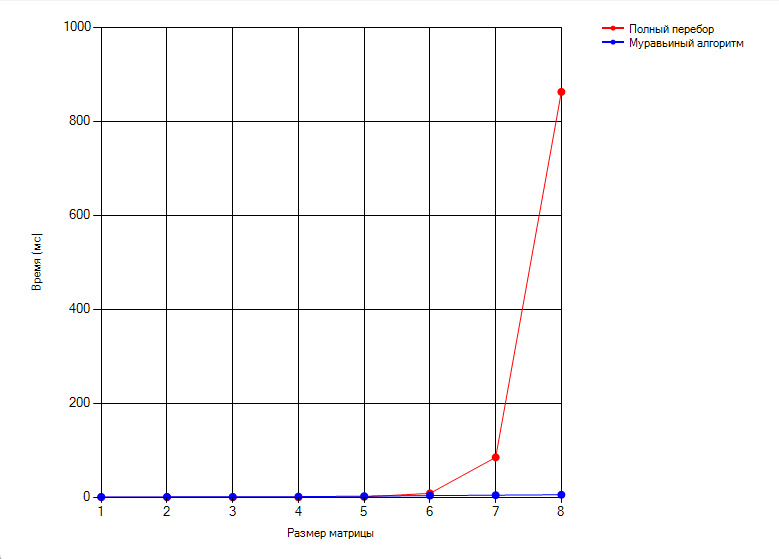
\includegraphics[width=1\linewidth]{img/graph-1.png}
    \caption{Зависимость времени выполнения программы от количества вершин}
    \label{fig:tm}
\end{figure}


\section{Классы данных}
В качестве класс данных для параметризации используются графы, построенные на городах Африке, при этом используется всего 3 графа. В качестве весов использовались расстояния между этими городами по прямой в км~\cite{maps}.

\section{Результаты параметризации}
В результате параметризации оказалось, что самыми лучшими параметрами по заданному классу данных оказались при $\alpha$ = 0.1, $\rho$ = 0.5 и количеством дней равным 50. При этом данные параметры дают лучший результат на всех классах данных и по всем параметрам сравнения. Результаты параметризации для лучших параметров представлены в таблице~\ref{tbl:param}, а
вся таблица параметризации и класс данных представлены в приложении А.


\begin{longtable}{|>{\centering\arraybackslash}r| >{\centering\arraybackslash}r| >{\centering\arraybackslash}r| >{\centering\arraybackslash}r| >{\centering\arraybackslash}r| >{\centering\arraybackslash}r| >{\centering\arraybackslash}r| >{\centering\arraybackslash}r| >{\centering\arraybackslash}r| >{\centering\arraybackslash}r| >{\centering\arraybackslash}r| >{\centering\arraybackslash}r|}
\caption{Результаты параметризации муравьиного алгоритма}\label{tbl:param}
\\ \hline
\multicolumn{3}{|c|}{Параметры} & \multicolumn{3}{|c|}{Граф 1} & \multicolumn{3}{|c|}{Граф 2} & \multicolumn{3}{|c|}{Граф 3} \\
\hline
$\alpha$ & $\rho$ & \text{Дни} & \text{min} & \text{max} & \text{avg} & \text{min} & \text{max} & \text{avg} & \text{min} & \text{max} & \text{avg} \\
\hline
\endfirsthead
\multicolumn{12}{c}{\text{Продолжение на следующей странице}} \\
\hline
\endhead
\hline
\multicolumn{12}{r}{\text{Конец таблицы}} \\
\hline
\endfoot
\endlastfoot
\hline
0.1 & 0.25 & 100 & 0 & 0 & 0 & 0 & 0 & 0 & 0 & 0 & 0 \\ 
0.1 & 0.25 & 200 & 0 & 0 & 0 & 0 & 0 & 0 & 0 & 0 & 0 \\ 
0.1 & 0.5 & 50 & 0 & 0 & 0 & 0 & 0 & 0 & 0 & 0 & 0 \\ 
0.1 & 0.5 & 100 & 0 & 0 & 0 & 0 & 0 & 0 & 0 & 0 & 0 \\ 
0.1 & 0.75 & 200 & 0 & 0 & 0 & 0 & 0 & 0 & 0 & 0 & 0 \\ 
0.25 & 0.1 & 100 & 0 & 0 & 0 & 0 & 0 & 0 & 0 & 0 & 0 \\ 
0.25 & 0.1 & 100 & 0 & 0 & 0 & 0 & 0 & 0 & 0 & 0 & 0 \\ 
0.5 & 0.1 & 200 & 0 & 0 & 0 & 0 & 0 & 0 & 0 & 0 & 0 \\ 
\hline
\end{longtable}


\textbf{ВЫВОД}

В результате исследования было получено, что на графе с вершинами меньше 7 муравьиный алгоритм и алгоритм полного перебора выполняют задачу за примерно одинаковое время, а при количестве вершин большем или равном 7 муравьиный алгоритм работает около в раз быстрее, чем алгоритм полного перебора.

Также было выявлено, что при $\alpha = 0.1$, $\rho = 0.5$ и количеством дней равным 50 муравьиный алгоритм дает наилучшие результаты.